\subsection*{Arrow Diagrams}
Sometimes the domain and codomain of a function are small, finite sets.  When this is the case, we can define a function simply by specifying the outputs for each input in the domain.  For example, if we let
 $A = \left\{ {1, 2, 3} \right\}$  and let  $B = \left\{ {a, b} \right\}$, we can define a function  
$F\x A \to B$ by specifying that 
\[
F( 1 ) = a, F( 2 ) = a, \text{ and }  F( 3 ) = b.
\]
%
This is a function since each element of the domain is mapped to exactly one element in  $B$.  A convenient way to illustrate or visualize this type of function is with a so-called \textbf{arrow diagram}
\index{arrow diagram}%
 as shown in Figure~\ref{fig:arrow61-1}.
\begin{figure}[h]
\begin{center}
\scalebox{0.85}[0.85]{
\includegraphics{figps-arrow61-1x.eps}} 
\caption{Arrow Diagram for a Function} \label{fig:arrow61-1}
\end{center}
\end{figure}
An arrow diagram can be used when the domain and codomain of the function are finite (and small).  We represent the elements of each set with points and then use arrows to show how the elements of the domain are associated with elements of the codomain.  For example, the arrow from the point  2  in  $A$  to the point  $a$  in  $B$  represents the fact that  $F( 2 ) = a$.  In this case, we can use the arrow diagram in 
Figure~\ref{fig:arrow61-1} to conclude that $\text{range} (F) = \{ a, b \}$.
\hbreak

\begin{prog}[\textbf{Working with Arrow Diagrams}] \label{pr:arrow} \hfill \\
Let  $A = \left\{ {1, 2, 3, 4} \right\}$ and let  $B = \left\{ {a, b, c} \right\}$.  
\begin{enumerate}
  \item Which of the arrow diagrams in Figure~\ref{fig:arrow61-2} can be used to represent a function from  $A$  to  $B$?  Explain. \label{exer:sec61-1}
  \item For those arrow diagrams that can be used to represent a function from $A$ to $B$, determine the range of the function.
\end{enumerate}
\begin{figure}[h]
\begin{center}
\scalebox{0.85}[0.85]{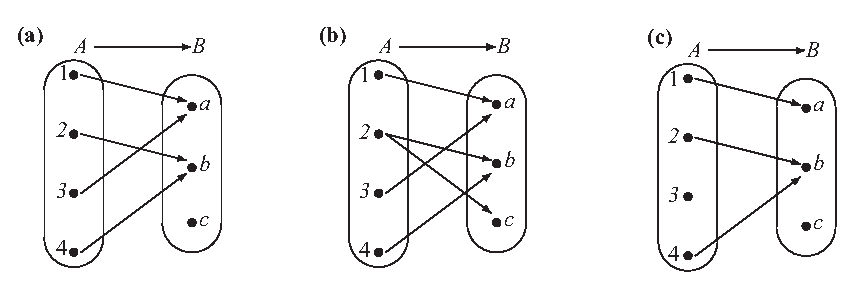
\includegraphics{figps-arrow-exer611abc.eps}} 
\caption{Arrow Diagrams} \label{fig:arrow61-2}
\end{center}
\end{figure}
\end{prog}
%\hbreak
\endinput
